[6~v\textsuperscript{o}] quantit\'{e} de la matiere\protect\index{Sachverzeichnis}{quantit\'{e} de la mati\`{e}re} qui le pousse.
Et par consequent cela ne feroit rien \`{a} la vitesse\protect\index{Sachverzeichnis}{vitesse}, tout de m\^{e}me comme la grandeur du corps.
Il s'ensuit donc que la division n'est pas la cause du retardement que nous voyons.
Il faut examiner par l'experience, si un corps pesant descend notablement plus doucement, quand il est contrebalanc\'{e} en partie, que si c'estoit la difference
\edtext{seule de deux qui}{\lemma{seule}\Bfootnote{\textit{(1)}\ qui \textit{(2)}\ de deux qui \textit{ L}}}
descend. L'experience peut estre rendue fort sensible en laissant tomber un corps sur une balance vuide de l'un cost\'{e} et remplie de l'autre, en sorte
\edtext{pourtant que}{\lemma{pourtant}\Bfootnote{\textit{(1)}\ qu'il \textit{(2)}\ que \textit{L}}}
celuy qui tombe soit plus pesant que celuy qui est en repos.
Si apr\`{e}s le \edtext{choc\protect\index{Sachverzeichnis}{choc} la vitesse}{\lemma{choc}\Bfootnote{\textit{(1)}\ le mouuement \textit{(2)}\ la vitesse \textit{L}}}
du tout est fort [diminu\'{e}e]\edtext{}{\Bfootnote{diminu\'{e}\textit{\ L \"{a}ndert Hrsg.}}}
(:~pourveu que la cause ne vienne pas du frottement\protect\index{Sachverzeichnis}{frottement} des pivots, ce qui se peut juger~:)
% \begin{wrapfigure}[7]{l}{0.4\textwidth}   
%    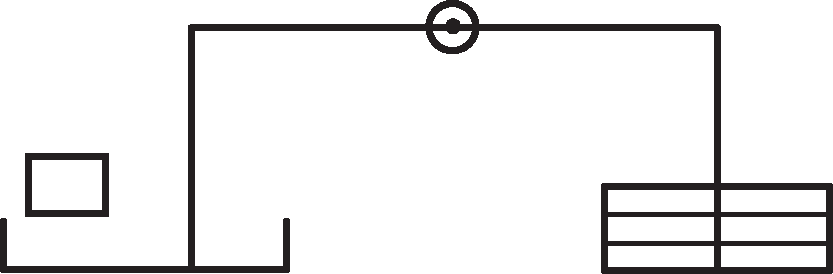
\includegraphics[trim = 0mm -6mm -5mm 0mm, clip, width=0.4\textwidth]{images/lh0350911_006v-d1.pdf}
%     \centering [\textit{Fig. 3}] % \caption{Bildbeschreibung}
%    \end{wrapfigure}
il en faut tirer la consequence, que la pesanteur\protect\index{Sachverzeichnis}{pesanteur} ne vient pas de la m\^{e}me cause d'o\`{u} vient
\edtext{[le]}{\lemma{}\Bfootnote{le \textit{erg.} \textit{Hrsg.}}}
retardement des balanciers\protect\index{Sachverzeichnis}{balancier} plus pesans.
Et on peut dire que les mouuemens visibles causent aussi la division d'une tout autre matiere que
\edtext{celle qui est caus\'{e}e par le mouuement}{\lemma{celle}\Bfootnote{\textit{(1)}\ que cause le mouuement \textit{(2)}\ qui est [...] mouuement \textit{L}}}
invisible interieur dans les corps pesans.
\pend
\count\Bfootins=1200
\count\Cfootins=1200
%\newpage
\pstart
Outre qu'il faut considerer qu'il y a dans le corps qui tombe, le mouuement acquis, qui ne vient plus de la pesanteur mais de la simple continuation du mouuement qu'on luy a donn\'{e}, comme quand on
\edtext{met un balancier}{\lemma{met}\Bfootnote{\textit{(1)}\ une pendule \textit{(2)}\ un balancier \textit{L}}}
ou autre chose en bransle et qu'on l'abandonne par apr\`{e}s.
Ce mouuement peut estre retard\'{e} par le mouuement d'une esp\`{e}ce de balancier equilibr\'{e} qui vient de la resistence\protect\index{Sachverzeichnis}{r\'{e}sistance} d'un autre corps;
\edtext{mais il ne s'ensuit pas de l\`{a} que l'impression m\^{e}me de la force}{\lemma{mais}\Bfootnote{\textit{(1)}\ la question est, si la fo \textit{(2)}\ il ne [...] l\`{a} que  \textit{(a)}\ le comm  \textit{(b)}\ l'impression m\^{e}me  \textit{(aa)}\ du corps pesant est p  \textit{(bb)}\ de la force \textit{L}}}
de la pesanteur est plus
\edtext{douce. En cas}{\lemma{douce.}\Bfootnote{\textit{(1)}\ Si \textit{(2)}\ En cas \textit{L}}}
qu'on trouue que les corps plus
\edtext{pesans vont aussi}{\lemma{pesans}\Bfootnote{\textit{(1)}\ marchent aussi \textit{(2)}\ vont aussi \textit{L}}}
viste par le principe de la pesanteur, que les moins pesans, et qu'une grande pendule\protect\index{Sachverzeichnis}{pendule} parcourt
\edtext{autant d'espace}{\lemma{autant}\Bfootnote{\textit{(1)}\ de temps \textit{(2)}\ d'espace \textit{L}}}
qu'une autre en autant de temps
([:]~\`{a} peu pr\`{e}s, ostant le retardement qui vient de l'air~:)
il s'ensuit que la pe-
\pend
\vspace{2em}
\pstart
\noindent
\centering
 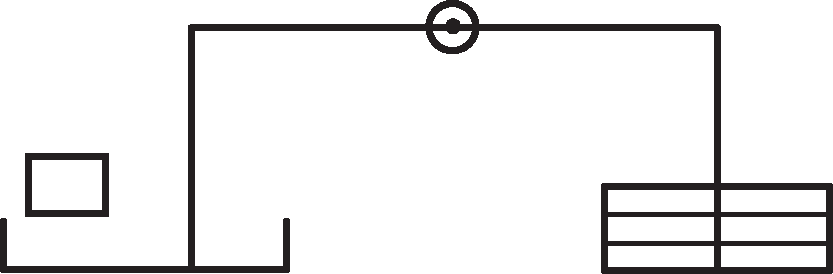
\includegraphics[trim = 0mm -6mm 0mm 0mm, clip, width=0.4\textwidth]{images/lh0350911_006v-d1.pdf}\\
     \centering [\textit{Fig. 3}] % \caption{Bildbeschreibung}
    \pend
\newpage
\count\Bfootins=1000
\count\Cfootins=1000
\pstart
\noindent
santeur et [ce]\edtext{}{\Bfootnote{se\textit{\ L \"{a}ndert Hrsg.}}} qui fait que les grands balanciers vont plus doucement que les petits, a son origine d'une m\^{e}me cause.
On pourra dire que la difference est insensible, mais nous voyons pourtant que celle des balanciers est fort sensible, et qu'ils marchent beaucoup plus doucement, quand ils sont grands.
Il est vray que le mouuement des balanciers n'est pas acceler\'{e}, et que celuy des pesans s'accelere, mais on peut pourtant remarquer au commencement des balanciers une grande difference.
NB. Il ne faut pas estimer la chose par la grandeur des pendules, mais il faut
\edtext{imaginer qu'un}{\lemma{imaginer}\Bfootnote{\textit{(1)}\ que \textit{(2)}\ qu'un \textit{L}}}
petit corps pesant fasse aller un grand balancier mais sans frottement, (comme
\edtext{celuy \edtext{d'Al\^{e}me:\protect\index{Namensregister}{\textso{D'Alême} (Dalême, Dalesme, d'Alesme), André 1725}%
}{\lemma{Al\^{e}me}\Cfootnote{%
Vermutlich der Uhrmacher und Maschinenbauer André d'Alême,\protect\index{Namensregister}{\textso{D'Alême} (Dalême, Dalesme, d'Alesme), André 1725} später \textit{pensionnaire méca\-nicien} der Pariser Akademie.
Keine von ihm vor 1686 veröffentlichten Schriften sind bekannt.
Er wird allerdings in Aufzeichnungen von C.~Huygens\protect\index{Namensregister}{\textso{Huygens} (Hugenius, Ugenius, Hugens, Huguens), Christiaan 1629-1695} genannt, die 1675 bis 1676 verfasst wurden und die Überschrift \cite{01164}\textit{Balancier de montre reglé par un ressort} tragen (\cite{00113}\textit{HO} VII, Nr.~2008, S.~413-415).
Möglicherweise fand zwischen Huygens und Leibniz Austausch über d'Alêmes technische Erfindungen statt.}}%
}{\lemma{celuy}\Bfootnote{\textit{(1)}\ de \textit{(2)}\ d'Al\^{e}me: \textit{L}}}
%\edtext{celuy d'Al\^{e}me}{\lemma{celuy}\Bfootnote{\textit{(1)}\ de \textit{(2)}\ d'Al\^{e}me \textit{L}}}\edtext{:}{\lemma{??Al\^{e}me}\Cfootnote{??Quelle nicht identifiziert.??}}
\edtext{ou le mien}{\lemma{ou}\Bfootnote{\textit{(1)}\ un lien \textit{(2)}\ le \textit{(3)}\ le mien \textit{L}}}
par le moyen d'un fil[)].
Ce qui se feroit fort simplement en attachant la pendule \`{a} un fil, en sorte qu'en mouuant le fil, elle remue un grand balancier qui y est attach\'{e}.
On verra si le mouuement du poids\protect\index{Sachverzeichnis}{poids} est plus doux quand le balancier est beaucoup plus grand.
Et on comparera ces deux forces ensemble, l'une qui cause le mouuement des corps pesans, l'autre qui fait que les balanciers plus pesans vont plus doucement.
Le balancier sera attach\'{e} \`{a} l'arbre suspendu entre deux fils.
Et c'est un moyen de faire aller doucement une pendule
[quoique]\edtext{}{\Bfootnote{quoque\textit{\ L \"{a}ndert Hrsg.}}}
fort courte, ce qui seroit d'un
\edtext{assez}{\lemma{}\Bfootnote{assez \textit{erg.} \textit{L}}}
grand usage, pour de petites pendules, et peut estre pour la mer, \`{a} cause que les grandes pendules y sont incommodes. [7~r\textsuperscript{o}]
\pend
\count\Bfootins=1500
%\newpage
\pstart
\vspace{1em}% PR: Provisorisch.